\documentclass{beamer}

\usepackage[italian]{babel}

\usetheme{default}

\author{Thomas Fossati}
\title{KINK\\ Interconnessione trasparente tra Web e IoT}
\institute{KoanLogic}

\begin{document}

\begin{frame}[plain]
  \titlepage
\end{frame}

\begin{frame}{Idea}
Trasformare ogni ``cosa'' (sensore, attuatore) in una \emph{risorsa informativa} integrata nella piattaforma Web, allo stesso modo in cui lo sono un articolo Wikipedia, un feed RSS, ecc.

\pause
\vspace{0.5cm}
Fornire lo strumento per integrare una (o pi\`u) WSN alla rete Internet in maniera \textbf{semplice} e \textbf{trasparente}.

\end{frame}

\begin{frame}{Vantaggi}
  \begin{itemize}
    \pause
    \item Riuso del middleware (Proxy, Cache, Origin Server)
    \pause
    \item Riuso delle interfacce uomo-macchina pi\`u diffuse (Browser, User Agent integrati)
    \pause
    \item Convergenza dei dati provenienti o diretti alle ``cose'' all'interno di un layer applicativo gi\`a molto ricco (mashup, azioni a distanza via API REST, ecc.).
  \end{itemize}
\end{frame}

\begin{frame}{Scenari d'uso}
  \begin{itemize}
    \pause
    \item Domotica
    \pause
    \item Controllo ambientale
    \pause
    \item Logistica
    \pause
    \item Health care
    \pause
    \item Trasporti
    \pause
    \item Energia
    \pause
    \item Convergenza nella cosiddetta ``Cloud''
  \end{itemize}
\end{frame}

\begin{frame}{Problema}
\begin{center}
Internet e Internet of Things sono due entit\`a distinte
\end{center}
\pause
\begin{center}
  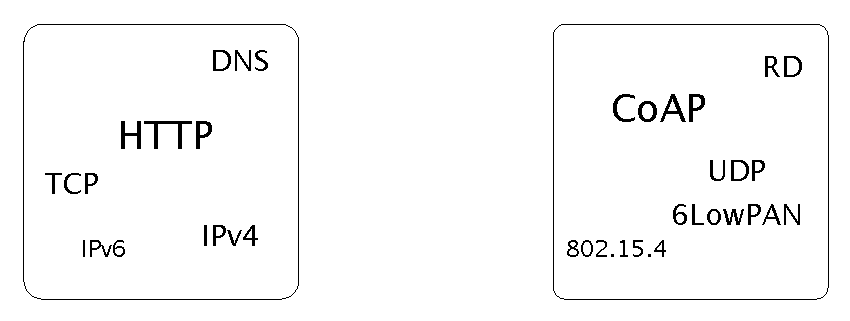
\includegraphics[width=0.7\textwidth]{images/schism.pdf} 
\end{center}
\end{frame}

\begin{frame}{Soluzione}
\begin{center}
KINK implementa il collante che le mette in comunicazione
\end{center}
\pause
\begin{center}
  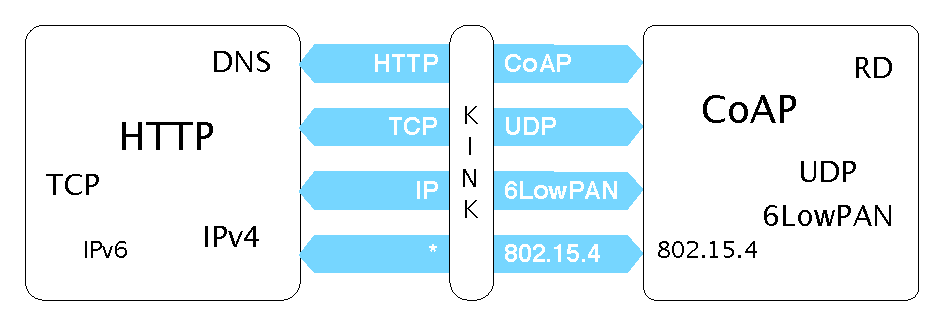
\includegraphics[width=0.7\textwidth]{images/join.pdf}
\end{center}
\end{frame}

\begin{frame}{KINK (Naming/Discovery)}
\begin{itemize}
  \pause
  \item Come chiamare le ``cose'' ?
  \pause
  \item Cosa bisogna rendere pubblico e come ?
  \pause
  \item Fino a che punto \`e possibile automatizzare le procedure ?
\end{itemize}
\end{frame}

\begin{frame}{KINK (Naming/Discovery)}
\begin{center}
Discovery automatica dei dispositivi (RD e CoRE link-format), traduzione URI, e pubblicazione via DNS o HTTP
\end{center}
\pause
\begin{center}
  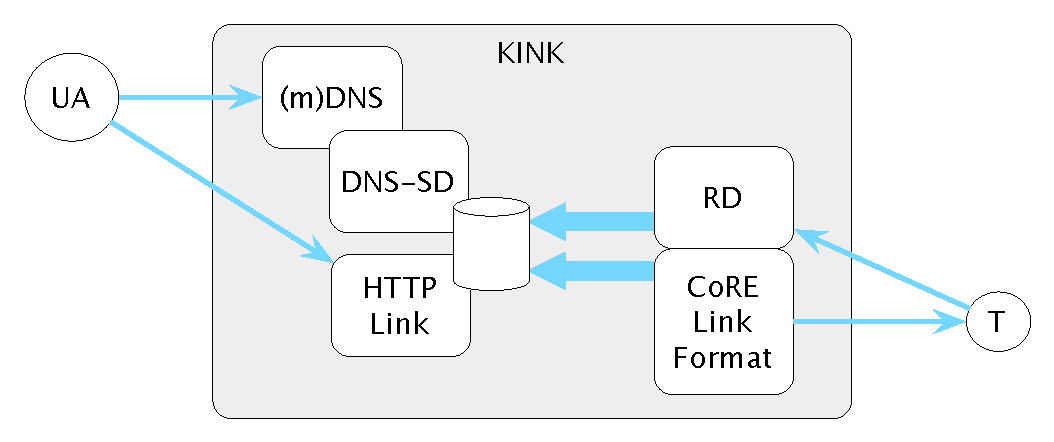
\includegraphics[width=0.7\textwidth]{images/discopub.pdf}
\end{center}
\end{frame}

\begin{frame}{KINK (Protocol Translation)}
\begin{itemize}
  \pause
  \item Cosa bisogna tradurre e in che modo ?
  \pause
  \item Fino a che punto \`e possibile mappare le semantiche ?
\end{itemize}
\end{frame}

\begin{frame}{KINK (Protocol Translation)}
\begin{center}
Traduzione automatica dello stack protocollare
\end{center}
\pause
\begin{center}
  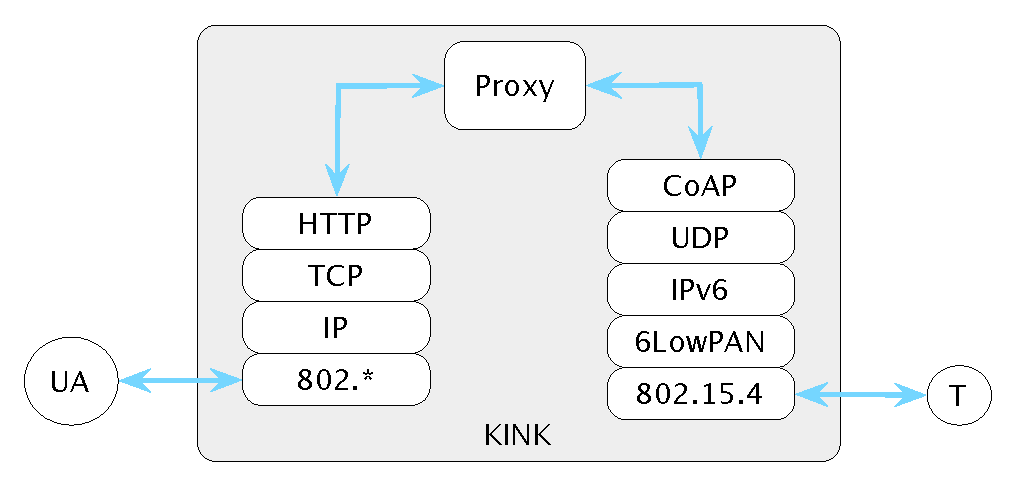
\includegraphics[width=0.7\textwidth]{images/trans.pdf}
\end{center}
\end{frame}

\begin{frame}{Tecnologie sviluppate ed integrate}
Comunicazione
\begin{itemize}
  \pause
  \item CoAP
  \pause
  \item HTTP
  \pause
  \item Caching
  \pause
  \item 6LowPAN
  \pause
  \item 802.15.4
\end{itemize}
\end{frame}

\begin{frame}{Tecnologie sviluppate ed integrate}
Discovery
\begin{itemize}
  \pause
  \item mDNS
  \pause
  \item DNS-SD
  \pause
  \item Link/HTTP
  \pause
  \item RD
  \pause
  \item CoRE Link Format
\end{itemize}
\end{frame}

\begin{frame}{Prodotto finale}
Un'unica software base, almeno quattro possibilit\`a di prodotto:
\begin{itemize}
  \pause
  \item Embedded standalone box (firmware basato su una distro OpenWRT custom)
  \pause
  \item Componenti software da integrare in una CPE (Linux/BSD) di terza parte
  \pause
  \item Immagine VM per data center che necessitano integrazione di ambienti eterogenei (things + web)
  \pause
  \item Integrazione dei componenti \emph{bridge} su smartphone (opportunistic proxy!)
\end{itemize}
\end{frame}

\begin{frame}{Stato dell'arte}
\begin{itemize}
  \pause
  \item Disegno architetturale concluso
  \pause
  \item Discreta quantit\`a di software gi\`a implementato e testato (non ancora pronto per ambiente di produzione)
  \pause
  \item Demo end-to-end (esclusa discovery) eseguita con successo
  \pause
  \item Test di interoperabilit\`a ETSI in programma per la fine di Marzo a Parigi
  \pause
  \item Build firmware in progettazione
  \pause
  \item Partecipazione attiva nei gruppi di lavoro IETF inerenti (HTTPbis e CoRE) con un buon numero di tecnologie proposte per la standardizzazione
\end{itemize}
\end{frame}

\begin{frame}{Prossimi passi}
\begin{itemize}
  \pause
  \item Conclusione delle attivit\`a legate alla fase 1 dello sviluppo (rilascio versione base)
  \pause
  \item Ricerca di uno o pi\`u soggetti che intendano co-finanziare il passaggio dalla fase prototipale all'industrializzazione del prodotto
  \pause
  \item Pianificazione della fase 2
  \begin{itemize}
    \pause
    \item Design Web API
    \pause
    \item Individuazione di scenari applicativi \emph{verticali} e possibili soggetti interessati 
    % ad esempio BTicino che vuole incorporare il KINK per interfacciare la sua proposta di prodotti domotica verso l'esterno
    \pause
    \item Frontend
    \pause
    \item Demo templating
  \end{itemize}
\end{itemize}
\end{frame}

\end{document}
